%%%%%%%%%%%%%%%%%%%%%%%%%%%%%% -*- Mode: Latex -*- %%%%%%%%%%%%%%%%%%%%%%%%%%%%
%% 09-01.tex --     Automated Software Engineering submission
%% Author          : Philip Johnson 
%% Created On      : Tue Jan 06 10:41:51 2009
%% Last Modified By: Philip Johnson
%% Last Modified On: Mon Jan 19 10:10:38 2009
%%%%%%%%%%%%%%%%%%%%%%%%%%%%%%%%%%%%%%%%%%%%%%%%%%%%%%%%%%%%%%%%%%%%%%%%%%%%%%%
%%   Copyright (C) 2009  Philip Johnson
%%%%%%%%%%%%%%%%%%%%%%%%%%%%%%%%%%%%%%%%%%%%%%%%%%%%%%%%%%%%%%%%%%%%%%%%%%%%%%%
%% 

\documentclass[smallextended]{svjour3}     % onecolumn (second format)
\usepackage{graphicx}
\usepackage{natbib}
\usepackage{url}             

\journalname{For submission to: Automated Software Engineering}

\begin{document}
\title{Operational Definition and Automated Inference of Test-Driven Development with Zorro}
\author{Hongbing Kou \and Philip M. Johnson \and Hakan Erdogmus}
\institute{Hongbing Kou and Philip M. Johnson \at 
           Collaborative Software Development Laboratory  \\
           Department of Information and Computer Sciences \\
           University of Hawaii \\
           Honolulu, HI 96822 \\
           Tel.: 808-956-3489\\
           Fax:  808-956-3548\\
           \email{hongbing@hawaii.edu} \\
           \email{johnson@hawaii.edu} \\
}
\institute{Hakan Erdogmus \at 
           Software Engineering Group,
           Institute for Information Technology  \\
           National Research Council \\
           Ottawa, ON K1V1R9 CANADA \\
           Tel.: 613-991-1018\\
           \email{hakan.erdogmus@nrc.gc.ca} \\
}

\date{January, 2009}

\maketitle

\begin{abstract}

Test-driven development (TDD) is a style of development named for its most
visible characteristic: the design and implementation of test cases prior
to the implementation of the code required to make them pass. Many claims
have been made for TDD: that it can improve implementation as well as
design quality, that it can improve productivity, that it results in 100\%
coverage, and so forth.  However, research to validate these claims has
yielded mixed and sometimes contradictory results.  We believe that at
least part of the reason for these results stems from differing
interpretations of the TDD development style, along with an inability to
determine whether programmers actually follow whatever definition of
TDD is in use.

Zorro is a system designed to automatically determine whether a developer
is complying with an operational definition of Test-Driven Development
(TDD) practices.  Automated recognition of TDD can benefit the software
development community in a variety of ways, from inquiry into the ``true
nature'' of TDD, to pedagogical aids to support the practice of test-driven
development, to support for more rigorous empirical studies on the
effectiveness of TDD in both laboratory and real world settings.

This paper describes the Zorro system, its operational definition of TDD,
the analyses made possible by Zorro, and three empirical evaluations of the
system.  Our research shows that it is possible to define an operational
definition of TDD that is amenable to automated recognition, and
illustrates the architectural and design issues that must be addressed in
order to do so.  Zorro has implications not only for the practice of TDD,
but also for software engineering ``micro-process'' definition and
recognition through its parent framework, Software Development Stream
Analysis.



\keywords{Test Driven Development \and Hackystat \and Process Measurement}
\end{abstract}

\section{Introduction}
\label{intro}

Substantial claims have been made regarding the effectiveness of
test-driven development (TDD). Evangelists claim that it naturally
generates 100\% coverage, improves refactoring, provides useful executable
documentation, produces higher code quality, and reduces defect rates
\citep{Beck:03}.  Unfortunately, the empirical research results have been
equivocal.  Some results are positive: \cite{Bhat:06} found that
introducing TDD at Microsoft decreased defect rates significantly in two
projects, and \cite{Maximilien:03} transitioned an IBM development team to
TDD with a 50\% improvement in quality. But other results are negative:
\cite{Muller:02} found that TDD resulted in less reliable software than the
control group. Yet other results vary regarding the quality and productivity benefits: 
for exmaple, \cite{Erdogmus:05} found that TDD software on average was of no
higher quality than the control group although some productivity advantage with TDD
was observed.

Why might the research results on TDD be so mixed?  We believe that part of
the reason stems from two methodological issues that impede both progress
on understanding TDD's current effectiveness and future improvements to the
technique. 

First, TDD is often defined in a relatively simplistic and ambiguous manner
using toy examples.  This can mislead developers into thinking that TDD
does not apply to their more complex development situations. It can also
lead to different organizations defining the practice of TDD in very
different ways.

Second, research on TDD suffers from the ``process compliance problem''.
In other words, the experimental designs do not have mechanisms in place to
verify that subjects who are supposed to be using TDD practices are,
indeed, using them.  The lack of control over process compliance in these
experiments means that differences in outcomes may be due, at least in
part, to variance in understanding what it means to do TDD, as opposed to
differences between the control and experimental groups. If compliance can be measured,
meaningful reference points that represent acceptable or idealized patterns
can be defined, and deviations, or distance,  from these patterns can be correlated
with productivity and quality outcomes. \cite{Erdogmus:05} stress the importance of gauging process
compliance in empirical studies of TDD. 

From a pedagogical point of view, emerging empirical evidence also supports the hypothesis that
tool guidance is helpful while learning or mastering TDD \cite{Mishali:08}. 
Thus process compliance information, abstracted at the right level and presented unobtrusively, 
may provide useful feedback to developers to allow them better leverage the benefits of TDD. 

To address these problems, we believe that the software research and
development community needs to agree upon at least one (if not more)
standard, operational definitions of TDD. Furthermore, these definitions
 allow for a practical way to assess compliance in both laboratory and
real-world settings. However the definitions must be robust enough to allow for a wide variety of behaviors, rather 
than strive to enforce a narrowly defined strict process. 

In this paper, we present Zorro, a system for automated recognition of TDD
practices.  In essence, Zorro gathers a stream of low-level developer
behaviors (such as invoking a unit test, editing production code, invoking
a refactoring operation) while programming in an IDE, partitions this event
stream into a sequence of development ``episodes''.  Then it applies a
rule-based system to determine the type of an episode from a set representing a wide variety of behaviors, 
whether or not the episode constitutes an
instance of a TDD practice according to the operational definitions encoded in the rules, and finally the extent of compliance with
these definitions through adherence metrics and summary charts. 
The need for 
robustness in accomodating variant behaviors is demonstrated empirically in a prior study by \citep{Mishali:08} 
 evaluating a tool for guiding TDD activities. In that study, many participants express disagreement with the
behaviors definitions that are too restrictive or narrow. Zorro overcomes this hurdle by providing a fine-grained categorization of possible 
behaviors and providing adherence metrics that represent a continuum rather than a dichotomy.

Zorro illustrates one approach to addressing the issues mentioned above
that hinder the research and practice of TDD today.  Automatic collection
and analysis of data makes Zorro practical for use in both laboratory and
real-world settings: once installed, there is no overhead on the developer
with respect to data collection.  Second, Zorro can be used to develop a
variety of operational definitions of TDD. A Zorro ``TDD definition''
consists of the set of developer behaviors that must be recorded, the
manner in which this timestamped stream of events are partitioned into
episodes, and the rules used to classify an episode according to TDD terminology and 
determine whether the episode is compliant with idealized TDD patterns.  By
providing a way to define an operational definition of TDD, Zorro addresses
the compliance problem by enabling researchers and practitioners to
precisely characterize the extent to which the given definition of TDD was
applied (or not) in any given development scenario.  Furthermore, Zorro's
episode-based approach to TDD recognition provides a more nuanced approach
to characterizing the use of TDD by developers: rather than a binary,
``all-or-nothing'' approach, Zorro enables TDD usage characterizations
based on percentages, such as ``Developer A used TDD 73\% of the time''.

Zorro has undergone initial empirical evaluation through classroom and
industry-based case studies.  The results from classroom studies indicate that Zorro is a viable
approach to automated TDD recognition. The industrial case study was inconclusive. 

This paper is organized as follows.  Section \ref{sec:RelatedWork} presents
work related to Zorro.  Section \ref{sec:zorro} presents the architecture and implementation of Zorro with examples. 
Section \ref{sec:validation} presents three empirical evaluation experiments we performed to validate the 
Zorro inference mechanism and gain insight into its strengths and weaknesses.  
Section \ref{sec:conclusions} summarizes the contributions and future directions for this research. 

\section{Related work}
\label{sec:RelatedWork}

\subsection{The practice of TDD}

Test-Driven Development \citep{Beck:03} is a software development 
best practice popularized by Extreme Programming \citep{Jeffries:00,Beck:00}. 
It is normally introduced as a very simple practice consisting of only two rules:

\begin{enumerate}
\item Write new code only if an automated test has failed.
\item Eliminate duplication.
\end{enumerate} 

An equally simple but more process-oriented description is the the 
``stop light'' metaphor \citep{Beck:03}: 
\begin{enumerate}
\item Red - Write a little test that does not work, and perhaps does not even compile at first.
\item Green - Make the test work quickly, committing whatever sins are necessary in the process.
\item Yellow (Refactor) - Eliminate all the duplication created by merely getting the test to work.
\end{enumerate}

Important characteristics of TDD practice, according to \citep{Beck:01,Beck:03},  include the following.

{\em Write the test first.}
This is the key characteristic of TDD. Some developers using TDD advocate that if you are using 
TDD, you should ``never write a line of production 
code without a broken test case.'' 
Although adherence to this extent is not always practiced, the principle captures the essence of TDD. 

{\em Short iterations.}
Quickly adding production code to make test pass is important
to TDD. An iteration should last a few seconds to 
several minutes only. If hours of work are needed to make a 
test pass, then this is a sign that the developer should have divided the programming 
task into smaller subtasks that could be solved in a shorter
period of time.

{\em Frequent refactoring.}
Code is consistently refactored in TDD to create the simplest
possible design. The existence of a suite of unit tests gives 
developers the ``courage'' to refactor the code

{\em Rapid feedback.}
Unit testing is usually supported by the XUnit
framework that is now available for most languages.
After new production code is added, developers should invoke
the unit tests to test it right away. This feedback should be available
within seconds or minutes. 

{\em One ball in the air at a time.}  In typical software development, the
developer tries to simultaneously balance several requirements, including
system structure design, algorithm choice, code efficiency, readability,
communication with other code, and so forth.  Martin Fowler is quoted as
describing that process as being like ``keeping several balls in the air at
once''.  In contrast, it is claimed that in TDD, the developer only keeps
``one ball in the air at once'' and concentrates only on that ball. For
example, in the development step, the developer only needs to make the test
pass without worrying about whether it is a good or bad design. In the
refactoring step, the developer only worries about what makes a good
design.

{\em The code should always work.} 
In TDD, developers should run 
all tests at the end of each iteration. If any test has failed, 
the developer should fix it right away. The fix should be easy because 
only a small amount of code is written in each iteration. If running 
all tests after an iteration is not feasible, the continuous 
integration can be set up to run them all once a day or several 
times a day. 

TDD advocates claim that adherence to this approach can simultaneously
improve both quality and productivity \citep{Beck:01,Janzen:05}.  Because
software quality is sometimes hard to quantify and not universal, TDD practitioners and researchers
often use code coverage as a precursor for software quality. The code developed
in TDD should have very high coverage since no production code is created without
a corresponding unit test. Some advocates advocate 100\% coverage, however this level may be hard 
or impossible to achieve in practice depending on the coverage criterion (method coverage is easy 
to achieve at 100\%, but perfect branch and path coverage are much more elusive). 

The claimed rationale for why TDD improves productivity is a bit more
complicated and controversial. Production code and test code are both software. Writing tests 
in advance is
part of the design process, and it often does not take a long time to write a
small test once certain low-level design decisions are made. 
If developers need to write same amount of test code, TDD
should save development time because less time is spent on tests than in
the traditional test last or ad-hoc development methods. Tests also provide visibility into progress 
and small tests written incrementally encourage finer task decomposition and better task focus. Regressing 
tests frequently allows production errors to be discovered early, thereby reducing costly snowball 
effects. In addition, TDD
users claim that the method reduces the overall amount of time spent on
debugging and rework and bug fixes following operational failure, with a resulting increase in overall long-term
productivity \citep{Williams:03}.

\subsection{Empirical evaluation of TDD}
\label{sec:related-empirical}

Much research work has been conducted on studying important outcomes of TDD
such as software quality and developer productivity in recent years. In
addition to anecdotal experience reports and case studies
\citep{George:04,Maximilien:03,Williams:03,Kaufmann:03,Edwards:04,Bhat:06,Damm:06,Sanchez:07,Janzen:08},
researchers have run controlled and quasi-controlled experiments
\citep{Muller:02,Matjaz:03,Erdogmus:05,Janzen:08,Madeyski:07,Siniaalto:07,Gupta:07} to compare TDD against other
development methods such as test last and ad hoc. We categorize the
research as ``academic'' or ``industrial'' depending upon whether the study
subjects are students or professional developers.

\subsubsection{Empirical evaluation in academic settings}

\cite{Muller:02} conducted a study in an XP class in
Germany to test TDD against traditional programming.  The acceptance tests
were provided to both the TDD group and the control group. Interestingly,
students in the TDD group spent more time but their programs were less
reliable than the control group.

\cite{Edwards:04} adopted TDD in a junior-level class to compare
whether students got more reliable code after the use of TDD and WEB-CAT,
an assignment submission system. It turned out that the students using TDD
reduced their defect rate dramatically (45\% fewer defects/KSLOC using a
proxy metric) after adopting TDD, and a posttest survey found that TDD
students were more confident of the correctness and robustness of their
programs.

Similarly, \cite{Kaufmann:03} conducted a pilot study
on implications of TDD in an advanced project-oriented software engineering
course. They also reported that TDD helped to improve software quality and
programmers' confidence.

\cite{Matjaz:03} designed a controlled experiment involving 38 students to compare TDD with
Iterative Test-Last approach (ITL), which is a slightly modified TDD
development process in the order of ``code-test-refactor''.  This study
found no notable difference between the two approaches.


\citep{Erdogmus:05} used the well-defined test-last
and TDD approaches as in \cite{Matjaz:03} to study the effectiveness of TDD through a controlled experiment. 
This study
concluded that TDD programmers wrote more tests per unit of programming
effort than test-last programmers. They found that test code tends to increase 
minimum software quality, but there was no 
difference between the average quality of the programs produced by the TDD 
and test-last groups. According to this study the TDD group achieved overall better productivity, although 
the difference was not statistically significant.

\citep{Madeyski:07} conducted a single-subject experiment in which the subject used successive TDD and traditional 
development in a Java/AspectJ project to develop a web-based conference management system.  The subject spent
112 hours to develop the system. Subject's productivity initially improved 87 to 177\% with TDD, but when TDD was 
withdrawn, productivity did not regress to its previous levels. 
 

\citep{Siniaalto:07} conducted an experiment with 13 students. The students 
had prior development experience in the industry. They were asked to develop a small mobicle stock market 
browser application in Java. The researchers evaluated the effect of TDD based on test coverage and design
quality. Test coverage was improved with TDD. As for design quality, cohesion appeared 
to improve, but the result was weak and the effect on coupling was inconclusive.

The experiment by \citep{Gupta:07} involved 22 students.
The subjects developed toy registration and ATM applications using Java, spending 20-55 hours to complete
the task. The researchers observed that overall productivity was improved with TDD, but quality results 
were inconclusive.

\citep{Janzen:08}'s two experiments with graduate and undergraduate students yielded consistent results on software quality.
One experiment used two teams of three students with 0-5 years of prior development experience 
and the other used a single team of three novices. The subjects developed programs of 800 to 1300
lines of Java code. TDD improved test coverage and resulted in programs with smaller modules, methods, and methods per class. The 
complexity of the programs as per two measures were also higher, but more dramatically so with undergraduate students. Coupling
and cohesion results were inconclusive.


\subsubsection{Empirical evaluation in industrial settings}

Several attempts have been made by researchers to study software quality
and developer productivity improvements of TDD in industrial settings.  

\cite{George:04} ran a set of structured experiments
with 24 professional pair programmers in three companies. Each pair was
randomly assigned to a TDD group or a control group to develop a bowling
game application. The final projects were assessed at the end of the
experiment.  They found that TDD practice appears to yield code with
superior external code quality as measured by a set of blackbox test cases,
and TDD group passed 18\% more test cases. However, the TDD group spent
16\% more time on development, which could have indicated that achieving
higher quality requires some additional investment of time. Interestingly,
and in the contrast to the empirical findings, 78\% of the subjects
indicated that TDD practice would improve programmers' productivity.

\cite{Maximilien:03} transitioned a software team
from an ad-hoc approach to testing to TDD unit testing practice at IBM, and
this team improved software quality by 50\% as measured by Functional
Verification Tests (FVT).

\cite{Williams:03} conducted another case
study in IBM to study TDD. Compared to a baseline project developed in a 
traditional fashion, the defect density of the project developed 
in TDD was reduced by 40\% as measured by functional verification and 
regression tests. The productivity was not impacted by the additional 
focus on producing test code. 

\cite{Geras:04} isolated TDD from other XP
practices, and investigated the impact of TDD on developer productivity and
software quality. In their research, TDD does not require more time but
developers in TDD group wrote more tests and executed them more frequently,
which may have led to future time savings on debugging and development.

Another study of TDD at Microsoft conducted by Bhat and Nagappan
\citep{Bhat:06} reported remarkable software quality improvement as 
measured in number of defects per KLOC. After introduction of TDD, 
project A (Windows) reduced its defects rate by 2.6 times, and project 
B (MSN) reduced its defect rate by 4.2 times, compared to the organizational
average. Reportedly, developers in project A spent 35\% more development
time, and developers in project B spent 15\% more development time, than
the developers in non-TDD projects spent.

\citep{Damm:06} conducted a longitudinal case studies lasting up to 1.5 years with 100 professionals at Ericsson. The professionals
developed components for mobile applications using C++ and Java. They observed that TDD reduced total project costs by 5-6\%, fault slip-through by 5-30\%, and 
avoidable fault costs by 55\%.  

\citep{Sanchez:07}'s longer, single case study at IBM lasted 5 years and involved 9-17 developers working on a medium-size device
driver with legacy components. Over this period of time, the researchers noted a 19\% increase in development effort with TDD in return 
for a 40\% increase in internal defect rates. 

\citep{Janzen:08}'s suite of three industrial experiments and one case study involving overlapping teams and individuals of three
subjects yielded moderately favorable results for TDD for test coverage and some size metrics, 
but were not consistent for complexity, coupling and cohesion metrics. All of the studies involved development of real-world J2EE applications
ranging from 800 to 50,000 lines of code. 
Test coverage was improved with TDD in all studies but one. TDD also consistently resulted in smaller modules and methods per class (the latter except
in one study), but not in 
smaller methods.


\subsection{A comparative analysis of TDD studies}

The research findings regarding the effect of TDD practices on software quality 
and developer productivity are mixed,  as shown in 
Tables \ref{tab:ControlledTDDResearch} (Controlled Studies) and \ref{tab:CaseStudyTDDResearch} (Case Studies). 
The study conducted at Microsoft \citep{Bhat:06} and the study conducted 
at the University of Karlsruhe \citep{Muller:02} are two extreme cases. In 
\cite{Bhat:06}, the developers improved software quality up to four 
times after adopting TDD. In comparison, the TDD group in \cite{Muller:02} 
yielded less reliable programs than the control group. 

\begin{table}[ht]
\caption{Controlled and Quasi-Controlled Empirical Experiments on TDD}
\begin{tabular}{|l|l|l|p{1.0in}|p{1.0in}|} \hline 
Investigator      & A/I & Subjs.	& Software Quality	& Developer Productivity \\ \hline
\cite{Janzen:08}  & I & teams of 1-3 & & TDD had better test coverage (except in one team) and smaller modules   & N/A \\ \hline
\cite{Janzen:08}  & A & 1-2 teams of 3 & & TDD had better test coverage, smaller methods and modules, and less complexity \% &  N/A \\ \hline
\cite{Madeyski:07}  & A & 1	& N/A & TDD had 87-177\% better productivity initially  \\ \hline
\cite{Siniaalto:07}  & A & 13	& TDD had 87-177\% better quality initially & N/A \\ \hline
\cite{Gupta:07}  & A & 22	& Inconclusive & Improved overall productivity\\ \hline
\cite{George:04}  & I & 24	& TDD improved test coverage, possibly reduced cohesion & N/A \\ \hline
\cite{Geras:04}   & I & 14	& TDD had better quality & No impact \\ \hline 
\cite{Kaufmann:03}& A &  8 & N/A	    & 50\% improvement \\ \hline
\cite{Erdogmus:05}& A & 35	& No change	  & Improved productivity \\ \hline
\cite{Muller:02}  & A & 19 & Less reliable, but better reuse	& No change \\ \hline
\cite{Matjaz:03}  & A & 38	& No change	  & No change \\ \hline
\end{tabular}
\label{tab:ControlledTDDResearch}
\end{table}

\begin{table}[ht]
\caption{Empirical Case Studies on TDD}
\begin{tabular}{|l|l|l|p{1.0in}|p{1.0in}|} \hline 
Investigator        & A/I      & Subjs.	& Software Quality	& Developer Productivity \\ \hline
\cite{Janzen:08}  & I & team of 3 & & TDD had better test coverage and smaller methods and modules; & N/A \\ \hline
\cite{Sanchez:07}& I &  9-17	& 30\% reduction in defect density & Increased effort 19\% \\ \hline
\cite{Damm:06}& I &  100	& 5-30\% reduction in fault slip-through, 55\% reduction in fault costs & Project cost increased by 5-6\% \\ \hline
\cite{Maximilien:03}& I &  9	& 50\% reduction in defect density	& Minimal impact \\ \hline
\cite{Williams:03}  & I & 9	& 40\% reduction in defect density	& No change \\ \hline
\cite{Bhat:06}      & A & 11	& 2-4 times reduction in defect density	& 35\% and 15\% more time \\  \hline
\cite{Edwards:04}   & A & 59	& 54\% fewer defects	& N/A \\ \hline
\end{tabular}
\label{tab:CaseStudyTDDResearch}
\end{table}


\subsection{Automated software process research}
\label{sec:related-automation}

Automated software process research systems are often top-down in nature:
they take a high-level description of a system process and use it to
constrain, control, or understand the actual development behaviors.
Process programming \citep{Sutton:95}, modeling \citep{Curtis:92} and
simulation \citep{Turnu:04,Jensen:05} are typical research methods for
studying software processes.  Process conformance, at least as performed by Zorro,
is a bottom-up process in which the actual development behaviors are
the input to, as opposed to the output from, the system.

Cook and Wolf \citep{Cook:95,Cook:96} developed a client-server system
named Balboa to automate the process discovery using finite state machine
(FSM). Balboa collects developers' invocations of Unix commands and CVS
commits to construct event streams. It then uses a neural network, a MARKOV
chain, and data mining algorithms to discover the FSM of software
processes. With Balboa, Cook and Wolf were able to reproduce the ISPW 6/7
process in their research.

\cite{Jensen:04,Jensen:05} simulated an automated approach to discover and
model the open source software development processes. They took advantage
of prior knowledge to discover the software development processes by
modeling the process fragments using a PML description. Their prototype
simulation found that they could detect unusually long activities and
problematic cycles of activities. They suggested that a bottom-up strategy,
together with a top-down process meta-modeling is suitable for automated
process discovery. 

For this research, we chose a rule-based system to study process
conformance of low-level software processes. Instead of asking process
experts to inspect the FSM of the executed process as Cook and Wolf did
\citep{Cook:95}, we converted the process knowledge into a set of rules and
used them to infer the software development behaviors. Our method is very
close to Jansen's and Scacchi's approach \citep{Jensen:04} except that we
used rules rather than PML for process descriptions.

\cite{Wang:04} argued that the empirical research of TDD suffers from the
construct validity problem (as is also the case in some other empirical
software engineering research) because it lacks process conformance. They
developed a prototype called ``TestFirstGauge'' to study the process
conformance of TDD by mining the in-process log data collected by
Hackystat.

TestFirstGauge aggregates software development data collected
by Hackystat to derive programming cycles of TDD. They used T/P ratio 
(lines of test code verse lines of production code), testing effort 
against production effort and cycle time distribution as the indicator 
of TDD process conformance. This project precedes the Zorro software 
system \citep{csdl2-06-02}, and in fact it stimulated our research interest 
in studying low-level software process conformance. Unlike the
prototype implementation of TestFirstGauge in VBA using an Excel
spreadsheet, Zorro is integrated into the Hackystat system for automation,
reuse, and flexibility using rule-based system \citep{Friedman-Hill:03}.


Similarly, \cite{Wege:04} also focused on automated support of TDD process
assessment, but his work has a limitation in that it uses the CVS history
of code. Developers typically do not commit on-going project data at the
granularity of seconds, minutes or hours, making this data collection
technique problematic for the purpose of TDD inference. At least for the
operational definition of TDD developed in this research, collecting rapid
low-level development activities is crucial to correctly identifying its
occurrence.

In their evaluation of TDD vs. test-last development, \cite{Madeyski:07} use a 
plugin for Eclipse 
\cite{ActivitySensor} in order to assess the subjects' compliance with the assigned development processes. 
Their plug-in is similar to TestFirstGauge and Zorro in that it records low-level developer activity data from the IDE, 
and caches the data in the local project directory. Then it makes automated commits to the project�s repository. 
For each commit, AS offers basic reports to developers as well as to the organizations
 for assessing activities involved in each commit. The plugin is said to
 achieve Zorro's and TestFirstGauge's reporting capabilities locally, without connecting 
to a HackyStat server. Further details about this tool is  unavailable.

TDDGuide by \cite{Mishali:08} 
is another process compliance tool that is integrated into the Eclipse IDE.
The main motivation behind TDDGuide is not assessment, but guidance, particularly when learning TDD. 
Unlike Zorro and TestFirstGauge, TDDGuide operates in real time to instantly detect and report compliant and non-compliant
patterns to respectively encourage and discourage the developer. It also has logging capability for off-line analysis.
Similar to Zorro, TDDGuide is rule-based, however it
operates at a higher level of granularity than Zorro, hence its classification scheme for identifying patterns is coarser and less
diverse than Zorro's. The tool reports any 
deviations from pre-defined TDD patterns to the developer and proposes activities for conformance. Most users who used the tool
to drive TDD activities in two experiments reported that TDDGuide helped them adhere to TDD behaviors, however about half of those
of users found the tool to be intrusive. TDDGuide, unlike Zorro and TestFirstGauge, does not produce adherence metrics and 
summary charts for visualizing developer activities.


\section{Zorro}
\label{sec:zorro}

\subsection{Architectural components}

As illustrated in Figure \ref{fig:ZorroArchitecture}, the Zorro
architecture consists of three subsystems: (1) Hackystat, which collects
low-level developer behaviors; (2) SDSA (Software Development Stream
Analysis), a Hackystat application that supports generic analysis of
development event streams; and (3) Zorro, an SDSA application, which
defines the specific rules and analyses necessary for recognition and
interpretation of the TDD behavior of a developer.

\begin{figure*}[th]
  \center
  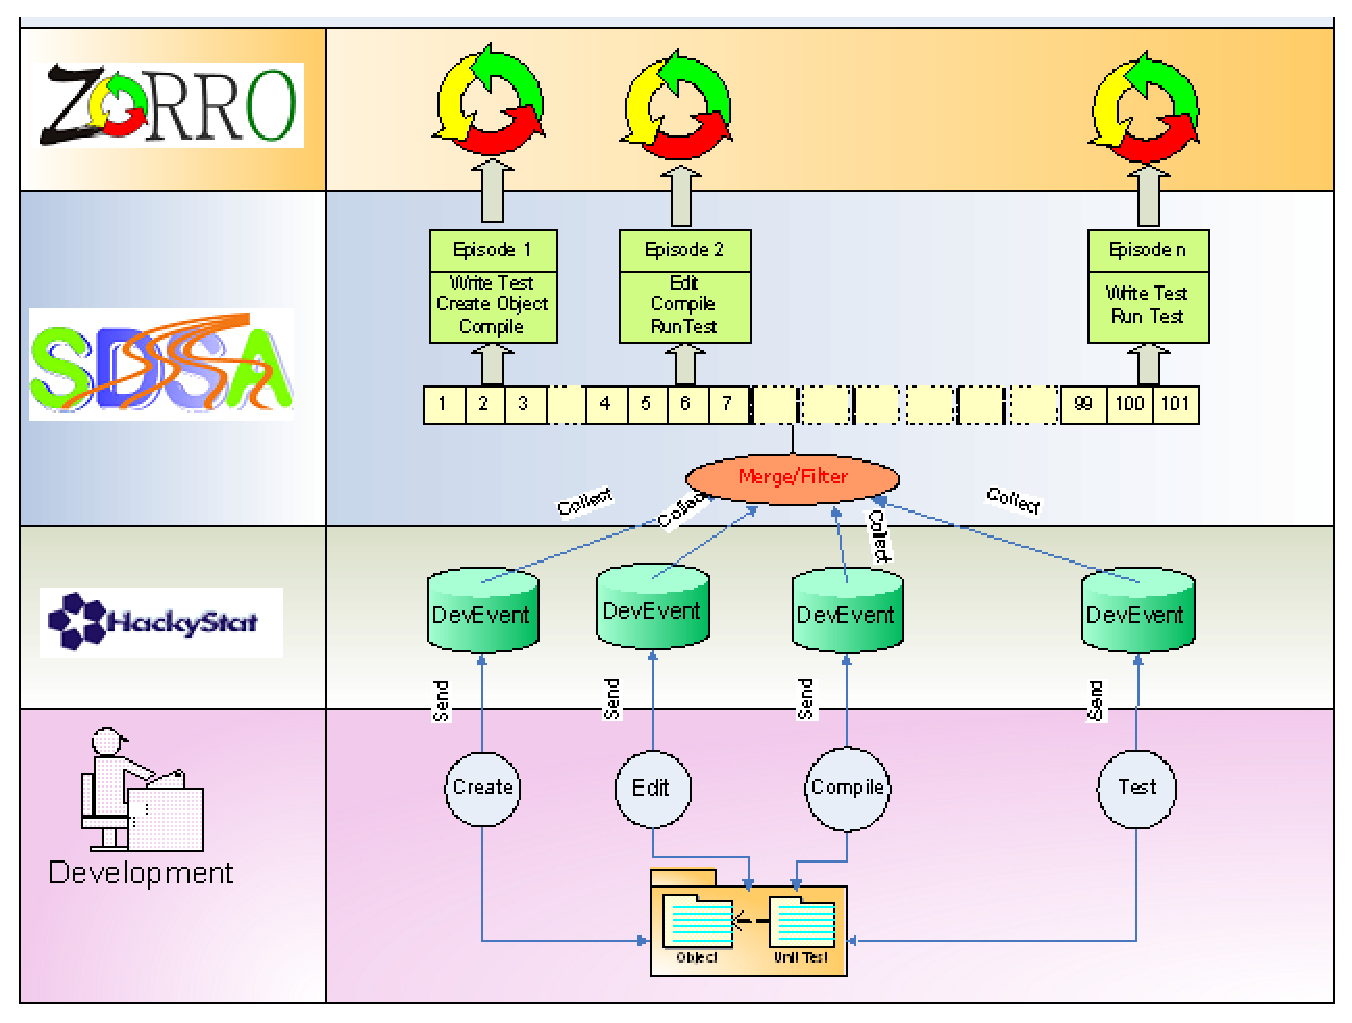
\includegraphics[width=1.0\textwidth]{zorro-architecture.eps}
  \caption{The Zorro Architecture}
  \label{fig:ZorroArchitecture}
\end{figure*} 


{\bf Hackystat.} Hackystat is an open source framework for automated
collection and analysis of software engineering process and product data
that we have been developing since 2001. Hackystat supports unobtrusive
data collection via specialized ``sensors'' that are attached to
development environment tools and that send structured ``sensor data type''
instances to a web-based Hackystat service for subsequent analysis.  Over
two dozen sensors are currently available, including sensors for IDEs
(Emacs, Eclipse, Vim, VisualStudio, Idea), configuration management (CVS,
Subversion), bug tracking (Jira, Bugzilla), testing and coverage (JUnit,
CppUnit, Emma, JBlanket), system builds and packaging (Ant), static
analysis (Checkstyle, PMD, FindBugs, LOCC, SCLC), and so forth.
Applications of the Hackystat Framework in addition to our work on SDSA and
Zorro include in-process project management \citep{csdl2-04-11}, high
performance computing \citep{csdl2-04-22}, and software engineering
education \citep{csdl2-03-12}.

Zorro requires the developer's IDE to be instrumented with a Hackystat
sensor that can collect at least the following kinds of events: unit test
invocations (and their results), compilation events (and their results),
refactoring events (such as renaming, moving), and editing (or code
production) events (such as whether the file has changed in state during
the previous 30 seconds, and what the resulting size of the file is in
statements, methods, and/or test case assertions).

We have implemented a Hackystat sensor for the Eclipse IDE to collect these
events for the Java language, and a Hackystat sensor for the Visual Studio
IDE to collect these events for the C\# language.


{\bf SDSA.} Software Development Stream Analysis (SDSA) is a Hackystat-based application that
provides a generic framework for organizing and analyzing the various kinds
of data received by Hackystat as input to a rule-based, time-series
analysis.

SDSA begins by merging the events collected by various sensors into a
single sequence, ordered by time-stamp, called the ``development stream''.
This is followed by a process called tokenizing, which results in a
sequence of higher-level ``episodes''.  These constitute the atomic
building blocks for whatever process is being recognized.  For any given
application of the SDSA framework, tokenization involving defining the
specific events to be combined to generate the development stream, as well
as the boundary condition that separates the final event in one episode
from the initial event in the next. For example, development events could
include things like a unit test invocation, a file compilation, a
configuration management commit, or a refactoring operation.  Example
boundary conditions could include a configuration management system
checkin, test pass event, or a buffer transition.

Once the development stream has been abstracted into a sequence of
episodes, the next step in SDSA is to classify each episode according to
whatever process is under analysis.  SDSA provides an interface to the JESS
rule-based system engine to enable developers to specify part or all of the
classification process as a set of rules.


{\bf Zorro.} The Zorro architectural layer provides extensions to Hackystat and SDSA
necessary for the automated recognition of Test Driven Development
behaviors.  Let's now examine Zorro's inferencing mechanism in more detail. 

\subsection{TDD Inference using Zorro: A simple example}

As introduced above, TDD inference in Zorro consists of the following
steps: (a) collection of low-level developer sensor data using Hackystat;
(b) abstraction of the sensor data into a developer event stream; (c)
partitioning of the event stream into episodes; and finally
(d) classification of the resulting episodes as either TDD-conformant or TDD
non-conformant.  Figure \ref{fig:SDSA-Example} illustrates an example of
the last three steps in this process.

\begin{figure}[htbp]
  \centering
  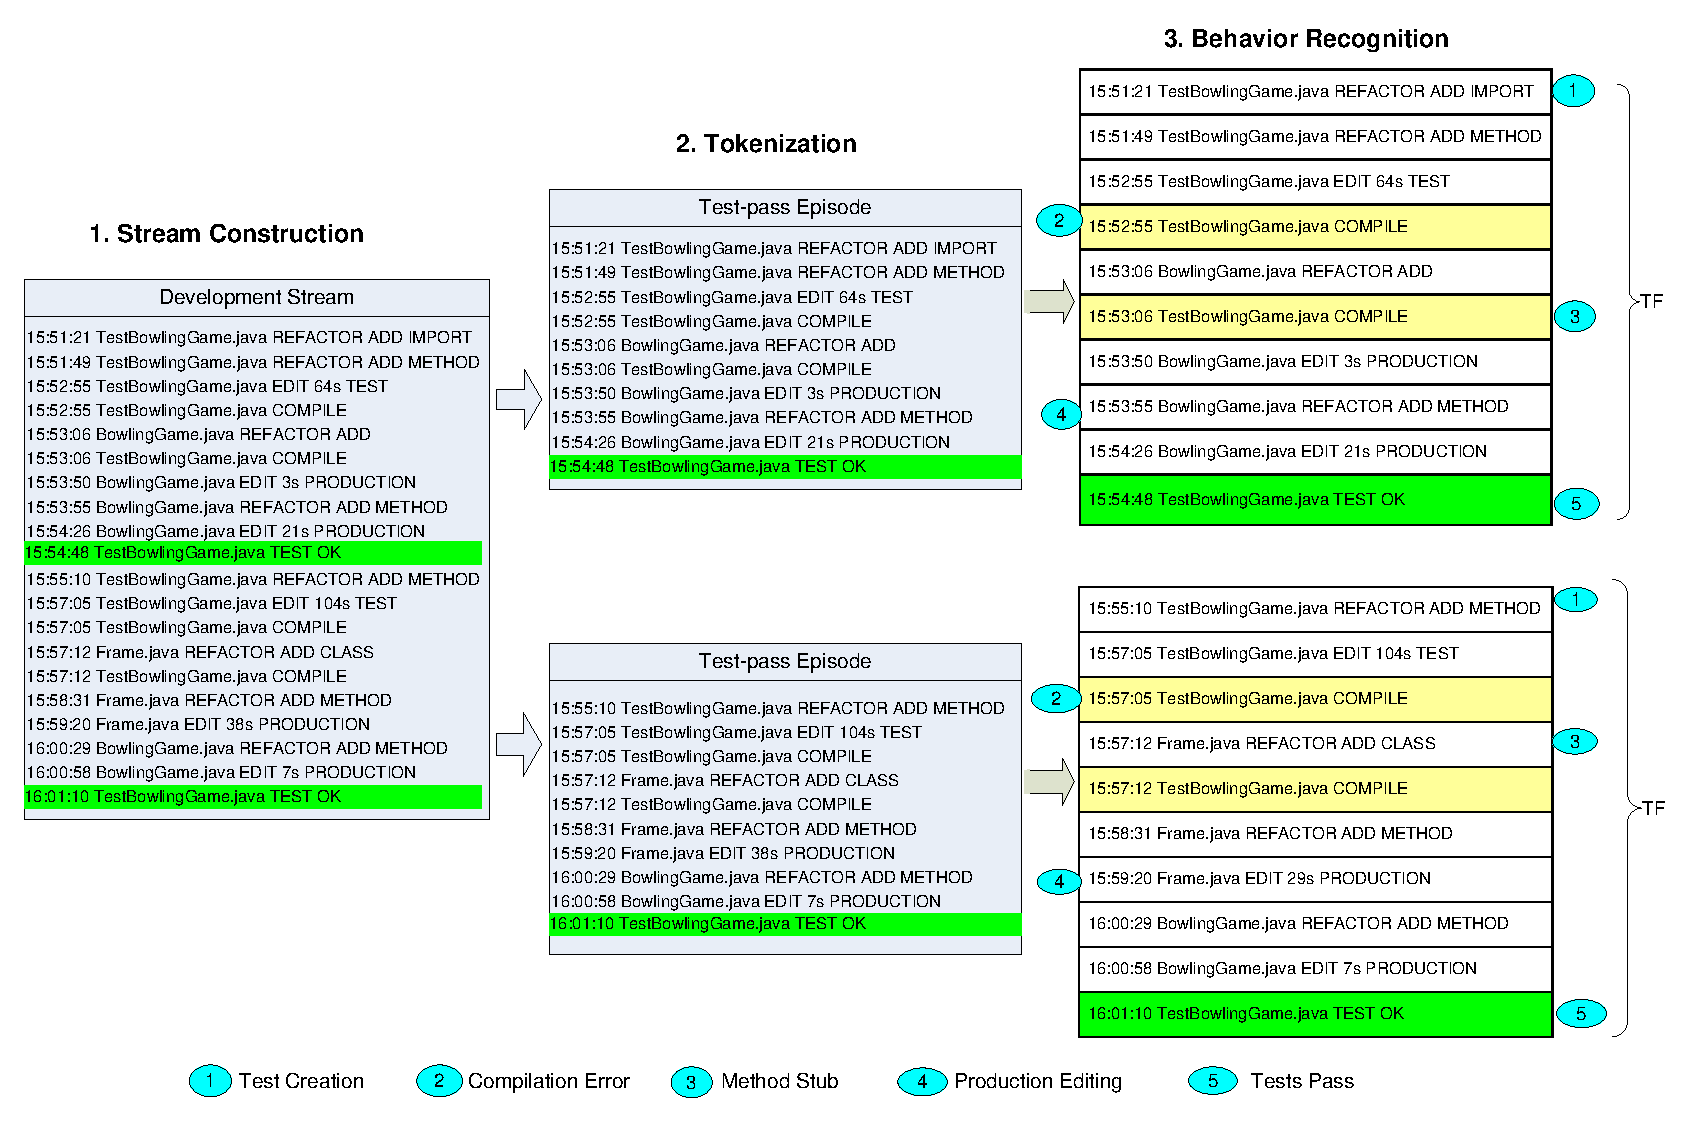
\includegraphics[width=1.0\textwidth]{Visio-SDSA-Example}
  \caption{Collecting, partitioning, and classifying developer behaviors}
  \label{fig:SDSA-Example}
\end{figure}

From 15:51:21 to 16:01:10, a developer implemented two user stories of the
bowling game in Test-Driven Development. We used Hackystat to instrument
the development process and collect sensor data regarding 
refactoring, editing, compilation and test invocation activities.  The ``Stream
Construction'' phase results in the consolidation of the raw Hackystat
sensor data into a sequence of 21 developer actions. Each action includes a
timestamp (such as 15:51:21), a file (such as ``TestBowlingGame.java''),
and an action type (such as ``EDIT 64s TEST'').

Among the 21 developer actions are two successful test invocation actions
(``TEST OK'').  Zorro partitions the stream of developer actions into
episodes based upon the occurrence of a successful test invocation action,
so this sequence of 21 actions is partitioned into two episodes, both
ending with a successful test invocation action.

The next step is to determine which, if any, of these two episodes
corresponds to a valid TDD development practice.  To do this, Zorro applies
a rule-based recognition system.  In this example, both episodes contain
the following sequence of actions: (a) a test method is created; (b) a
compilation error results; (c) a method stub is created in production code
which results in a successful compile; (d) more production code is edited;
and (e) all tests pass.  These actions correspond to the classic style of
TDD development, and Zorro's rules will classify both of these episodes as
instances of TDD.

Of course, in the case of simple toy examples where a developer follows the
canonical TDD approach, it is not surprising that Zorro can identify the
behavior as TDD.  The more important issue is how to deal with the
complexities of real world software development behaviors. 

\subsection{Episode classification}

The heart of Zorro is its episode classification algorithm, implemented as
a set of JESS rules.  Figure \ref{fig:Categories} summarizes the effect of these rules, 
which is to classify any episode as belonging to one of 22 episode types. 

\begin{figure*}[th]
  \center
  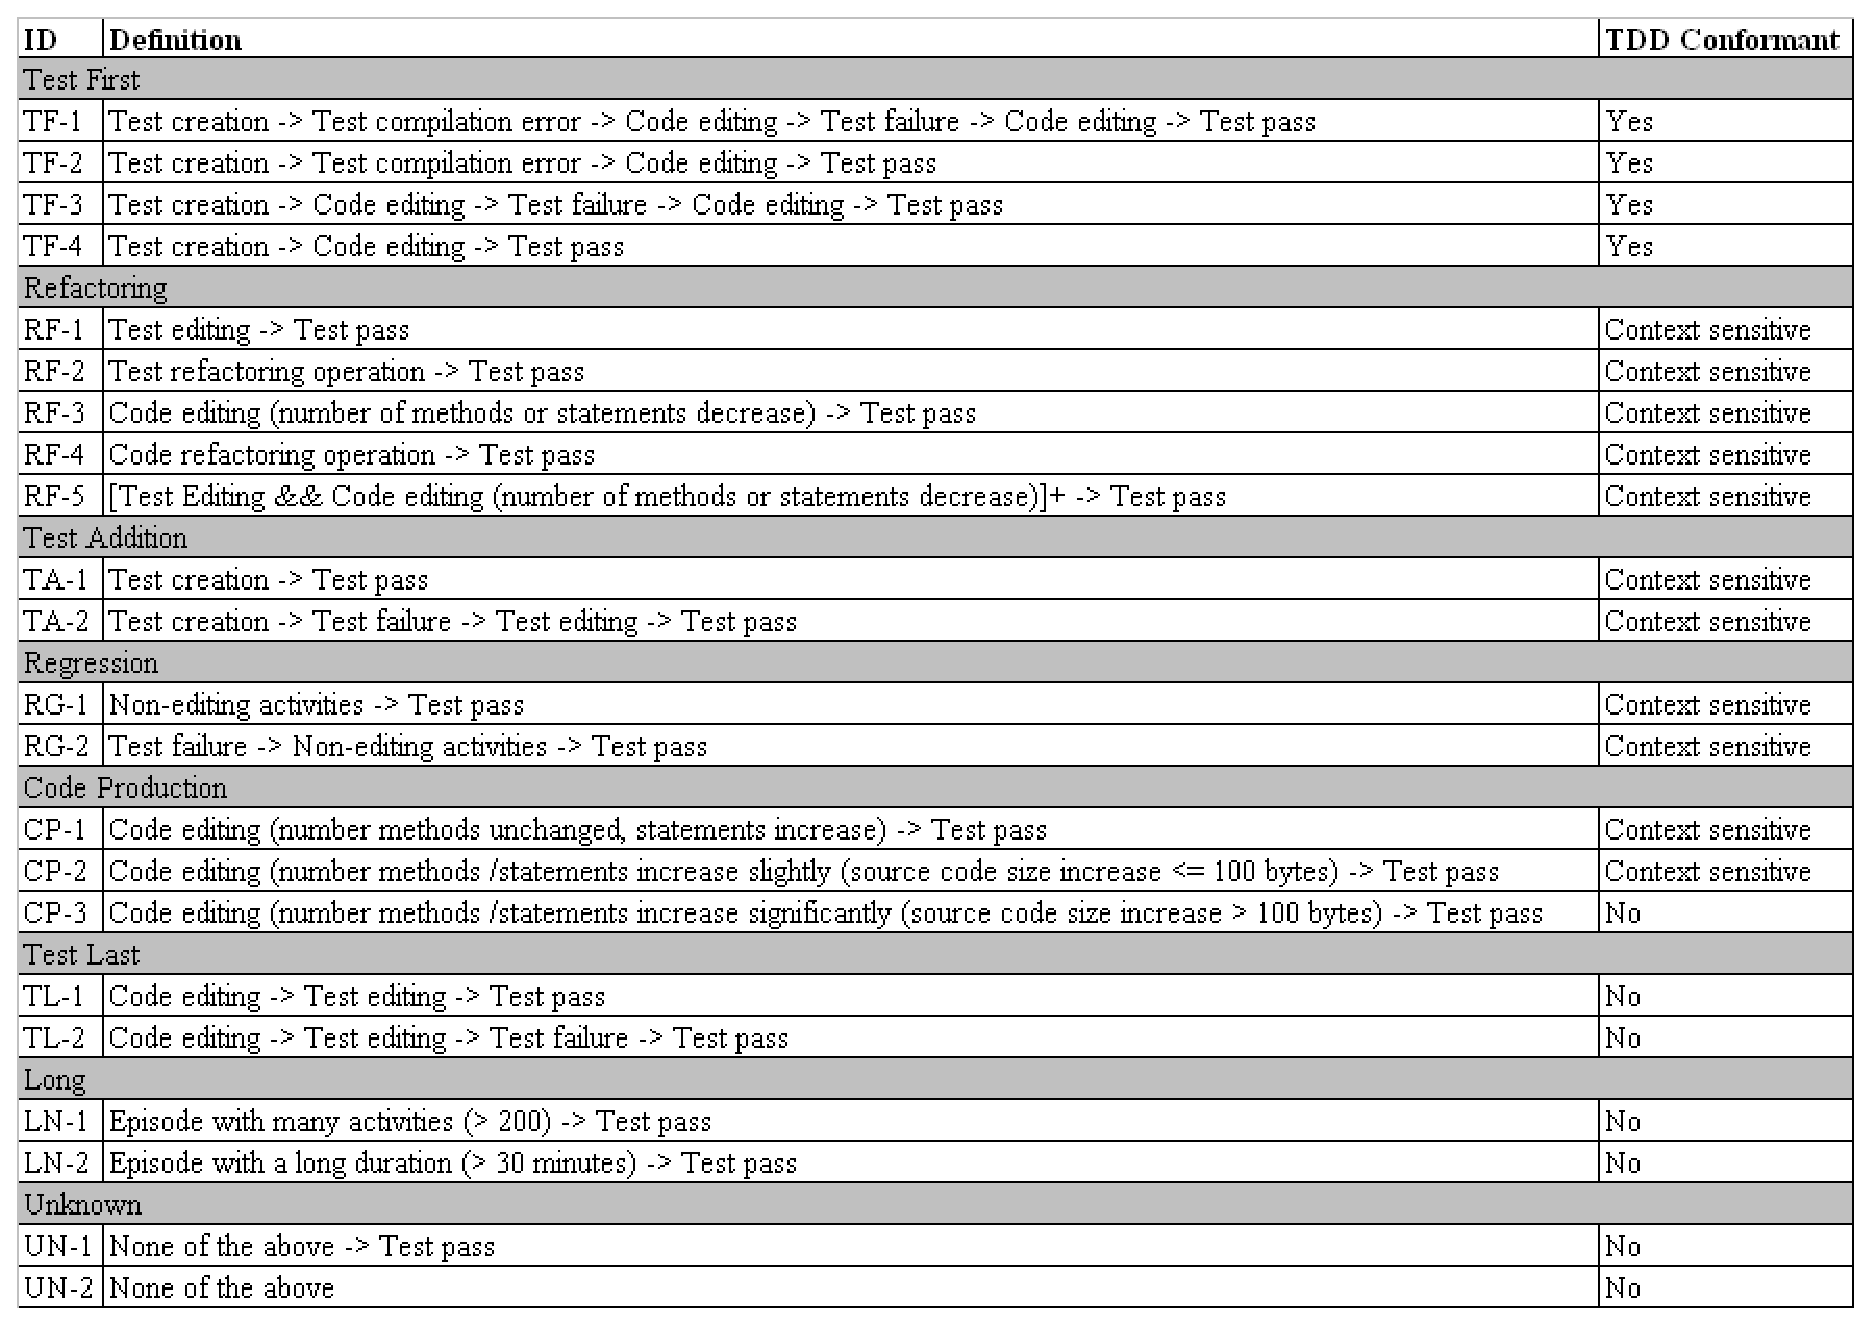
\includegraphics[width=1.0\textwidth]{episode-classification.eps}
  \caption{Zorro episode types, definitions, and TDD conformance}
  \label{fig:Categories}
\end{figure*} 

Zorro organizes the 22 episode types into eight categories: Test First
(TF), Refactoring (RF), Test Last (TL), Test Addition (TA), Regression
(RG), Code Production (CP), Long (LN), and Unknown (UN).  All of these
episode types (except UN-2) always ends with a ``Test pass'' event, since that
is the episode boundary condition.  (UN-2 is provided as a way to classify
a development session where there is no unit testing at all.) 

The definition column 
gives a typical instance for each an episode category. The implementation 
allows repetitions of certain sub-patterns inside each episode category as 
required. For example, the ``Code editing -> Test failure'' subpattern can be 
repeated one or more types inside 
an episode of category TF-1 although the instance shown 
in Figure \ref{fig:Categories} under the definition column
has a single occurrence of this sub-pattern.

Once each episode instance has been assigned an episode type by the SDSA
rule set, the final step in the Zorro classification process is to
determine the TDD conformance of that instance.  Figure
\ref{fig:Categories} shows that exactly half of the 22 episode types can be
unambiguously characterized as either TDD conformant or TDD non-conformant.
For example, all four Test First episode types are automatically TDD
conformant, just the seven Test Last, Long and Unknown episode
types are automatically TDD non-conformant.

An interesting discovery from our research is that only half of the episode
types we designed could be unambiguously characterized with respect to TDD
compliance.  The remaining episode types, including Refactoring, Test
Addition, Regression, and certain Code Productions are ambiguous: in
certain contexts, they could be TDD conformant, while in other contexts
they could be TDD non-conformant.  Consider the ``Refactoring'' episode
type.  Code refactoring can occur when a developer is doing Test Driven
Design, but it can just as easily occur when a developer is doing some
other style of development, such as Test Last programming.  In order to
classify instances of these ambiguous episode types, Zorro applies the
following heuristic: if a sequence of one or more ambiguous episodes are
bounded on both sides by non-TDD conformant episodes, then the ambigous
episode(s) are classified as non-TDD conformant. Otherwise, they are
classified as TDD conformant.

To make this clear, let's consider some examples.  For the episode sequence
[TF-1, RF-1, CP-1, TF-2], Zorro classifies the interior two ambiguous episodes (RF-1 and
CP-1) as TDD conformant, since they are surrounded by TDD conformant
episode types (TF-1 and TF-2).  Now consider the sequence [TL-1, RF-1,
CP-1, TL-2].  In this sequence, Zorro classifies the same two interior 
episodes as TDD non-conformant, since they are surrounded
by non-TDD episode types (TL-1 and TL-2).

Now consider a sequence like: [TF-1, RF-1, CP-1, TL-1].  Here, the two
interior ambiguous episodes (RF-1 and CP-1) are surrounded on one side by an
unambiguous TDD conformant episode (TF-1) and on the other side by an
unambiguous non-TDD episode (TL-1).  In this case, Zorro's rules
could implement an ``optimistic'' classification, and assign the interior ambiguous
episodes as TDD conformant, or a ``pessimistic'' classification, and assign
the interior ambiguous episodes as non-TDD.  The current Zorro definition
of TDD implements the ``optimistic'' classification for this situation.

The Zorro classification system illustrates two important advances in our
approach to TDD.  First, it replaces the simplistic ``red-green-yellow''
three episode type approach to TDD developer behavior with a much more
sophisticated classification scheme based upon 22 distinct episode
types. Second, it reveals that the mapping from developer behaviors to TDD
is not straightforward. One can reasonably question whether the
``optimistic'' classification scheme currently chosen for Zorro is ``correct'' or 
reflects
standard or recommended practice.  
The resolution to this question, and indeed to questions regarding any
chosen operational definition of TDD, is {\em validation}: the process of
gathering evidence to determine whether the chosen definition matches
reasonable expectations for what constitutes TDD and what doesn't. \citep{Mishali:08}'s 
evaluation of their TDD guiding tool  
suggests that reaching consensus among developer about what consitutes valid
TDD behavior may be difficult. 
We will return to this issue in Section \ref{sec:validation}.

\subsection{The user interface}

No matter how effective the classification mechanism, the usefulness of Zorro still depends upon a user interface that can help people understand how Zorro is performing its classification, and what the implications of TDD practice might be. 
This section overviews a few of the
analyses provided by Zorro to provide a flavor for what is possible with
this approach. For more details, see \cite{csdl2-07-04} and \cite{Wang:04}.

The first analysis, illustrated in Figure \ref{fig:Analysis-Table}, is
designed to provide transparency regarding the Zorro data collection and
classification process.

\begin{figure*}[th]
  \center
  \includegraphics[width=1.0\textwidth]{zorro-episode-interface.eps}
  \caption{Zorro Classification Analysis}
  \label{fig:Analysis-Table}
\end{figure*} 

Figure \ref{fig:Analysis-Table} displays two episodes, the first containing
19 development stream events and the second containing 10 development
stream events.  The display of each event includes its time-stamp, its
associated file (if applicable), and some additional information about the
associated sensor data.  The final column provides information about {\em
how} Zorro classified the episode (as either TDD conformant, or TDD
non-conformant), as well as {\em why} Zorro classified the episode that way
(via a textual summary of the episode structural characteristics used in
the classification).  

The analysis in Figure \ref{fig:Analysis-Table} is useful for those wishing
to understand Zorro's operational definition of TDD in the context of
actual development, either for learning or validation purposes.  Figure
\ref{fig:Analysis-Demography} provides a higher level perspective, by
showing only the sequence of episode types, with each TDD conformant
episode shaded in green. Clicking on an episode type drills down to a more
detailed description similar to that shown in Figure
\ref{fig:Analysis-Table}.

\begin{figure*}[th]
  \center
  \includegraphics[width=1.0\textwidth]{zorro-episode-demography.eps}
  \caption{Zorro Episode Demography}
  \label{fig:Analysis-Demography}
\end{figure*} 

Zorro provides a number of additional analyses that enable the developer to
understand the impact of TDD practices on their software product and
process.  Figure \ref{fig:Analysis-Ratio} shows how the ratio of test code
to non-test (production) code changes during the course of a development
session.  The horizontal bar at 1.0 represents equal amounts of test and
production code.  This figure illustrates a scenario of initial module
development in which there was significantly more production code than test
code at the beginning of the session, but the proportion of test code rose
until it doubled the amount of production code, before returning to 1.5
times the production code at the end of the session.

\begin{figure*}[th]
  \center
  \includegraphics[width=1.0\textwidth]{zorro-test-production-size-ratio.eps}
  \caption{Zorro Test/Production Size Ratio}
  \label{fig:Analysis-Ratio}
\end{figure*} 

The final example analysis illustrated in Figure
\ref{fig:Analysis-Telemetry} pops up to yet another level of abstraction by
using Software Project Telemetry, a capability of Hackystat that enables
the visualization of trends in process and product data over days, weeks,
or months.  In this real world data, two trends are displayed over the
course of eight weeks: the percentage of TDD conforming episodes, and the
test case coverage of the system under development.  Interestingly, the
level of test case coverage co-varies with the ``level'' of TDD practiced
by the developer.

\begin{figure*}[th]
  \center
  \includegraphics[width=1.0\textwidth]{zorro-tdd-coverage-2.eps}
  \caption{Zorro TDD Episode Telemetry}
  \label{fig:Analysis-Telemetry}
\end{figure*} 


\section{Empirical validation and evaluation}
\label{sec:validation}

In order to feel confident in Zorro as an appropriate tool to investigate
TDD, we must address two basic validation questions: (1) Does Zorro collect
the behaviors necessary to determine when TDD is occurring, and (2) Does
Zorro correctly recognize test-driven development when it is occurring?

The first validation issue addresses the use of automated, unobtrusive,
sensor-based data collection, and whether this approach can actually
acquire the data necessary to determine when TDD is taking place.

The second validation issue addresses our operational definition of TDD
based upon episode-based classification, and whether it provides a robust,
useful, and acceptable definition of TDD.

An important experimental design issue in the validation of Zorro is the
need to obtain an independent source of data regarding developer behaviors
apart from the Hackystat sensor data itself.  Without this independent
source of data, we could not verify that the sensor data was capturing
all relevent aspects of developer behavior, or even verify that the sensor
implementation was correct.

One approach to independent data collection is to have an observer
watching the developers as the program, and take notes as to whether they
are performing TDD or not.  We considered this approach but discarded it as
unworkable: given the rapidity with which TDD cycles can occur, it would be
quite hard for an observer to note all of the TDD-related events that can
occur literally within seconds of each other. We would effectively need to
validate our validation technique!

Instead, we developed a plugin to Eclipse called the ``Eclipse Screen
Recorder'' (ESR) \cite{esr}.  This system generates a Quicktime movie
containing time-stamped screen shots of the Eclipse window at regular
intervals. One frame/second was found to be sufficient for validation,
generating file sizes of approximately 7-8 MB per hour of video.  The
Quicktime movie created by ESR provides an independent, fine-grained,
accurate, and visual record of developer behavior that can be manually
compared to the Zorro analysis using the timestamps and used to address
validation questions.

The following sections summarize the three validation experiments we performed;
full details are available in \cite{csdl2-07-04}.

\subsection{Experiment 1: Classroom pilot study}

{\bf Goals.}  To obtain initial validation data on Zorro, we conducted a
short pilot study in Spring of 2006. The goal of this study was to ensure
that our data collection and analysis methodology was appropriate and
effective.

{\bf Procedure.}  We obtained agreement from seven volunteer student
subjects to participate in the pilot study. These subjects were experienced
with both Java development and the Eclipse IDE, but not necessarily with
test-driven development. 

We then provided them with a short description of test-driven design,
and a sample problem to implement in a test-driven design style.  The
problem was to develop a Stack abstract data type using test-driven design,
and we supplied them with an ordered list of tests to write and some sample
test methods to get them started.  Finally, they carried out the task using
Eclipse with both ESR and Zorro data collection enabled.

To analyze the data, we created a spreadsheet in which we recorded the
results of watching the Quicktime movie and manually encoding the developer
activities that occurred.  Then, we ran the Zorro analyses and added their
results to the spreadsheet.  Figure \ref{fig:VideoExcelScript} illustrates 
a portion of such a spreadsheet for one subject: the first column contains
the Zorro inferences, while the remaining columns contain manually analyzed
data from the ESR video.

\begin{figure}[htbp]
  \centering
  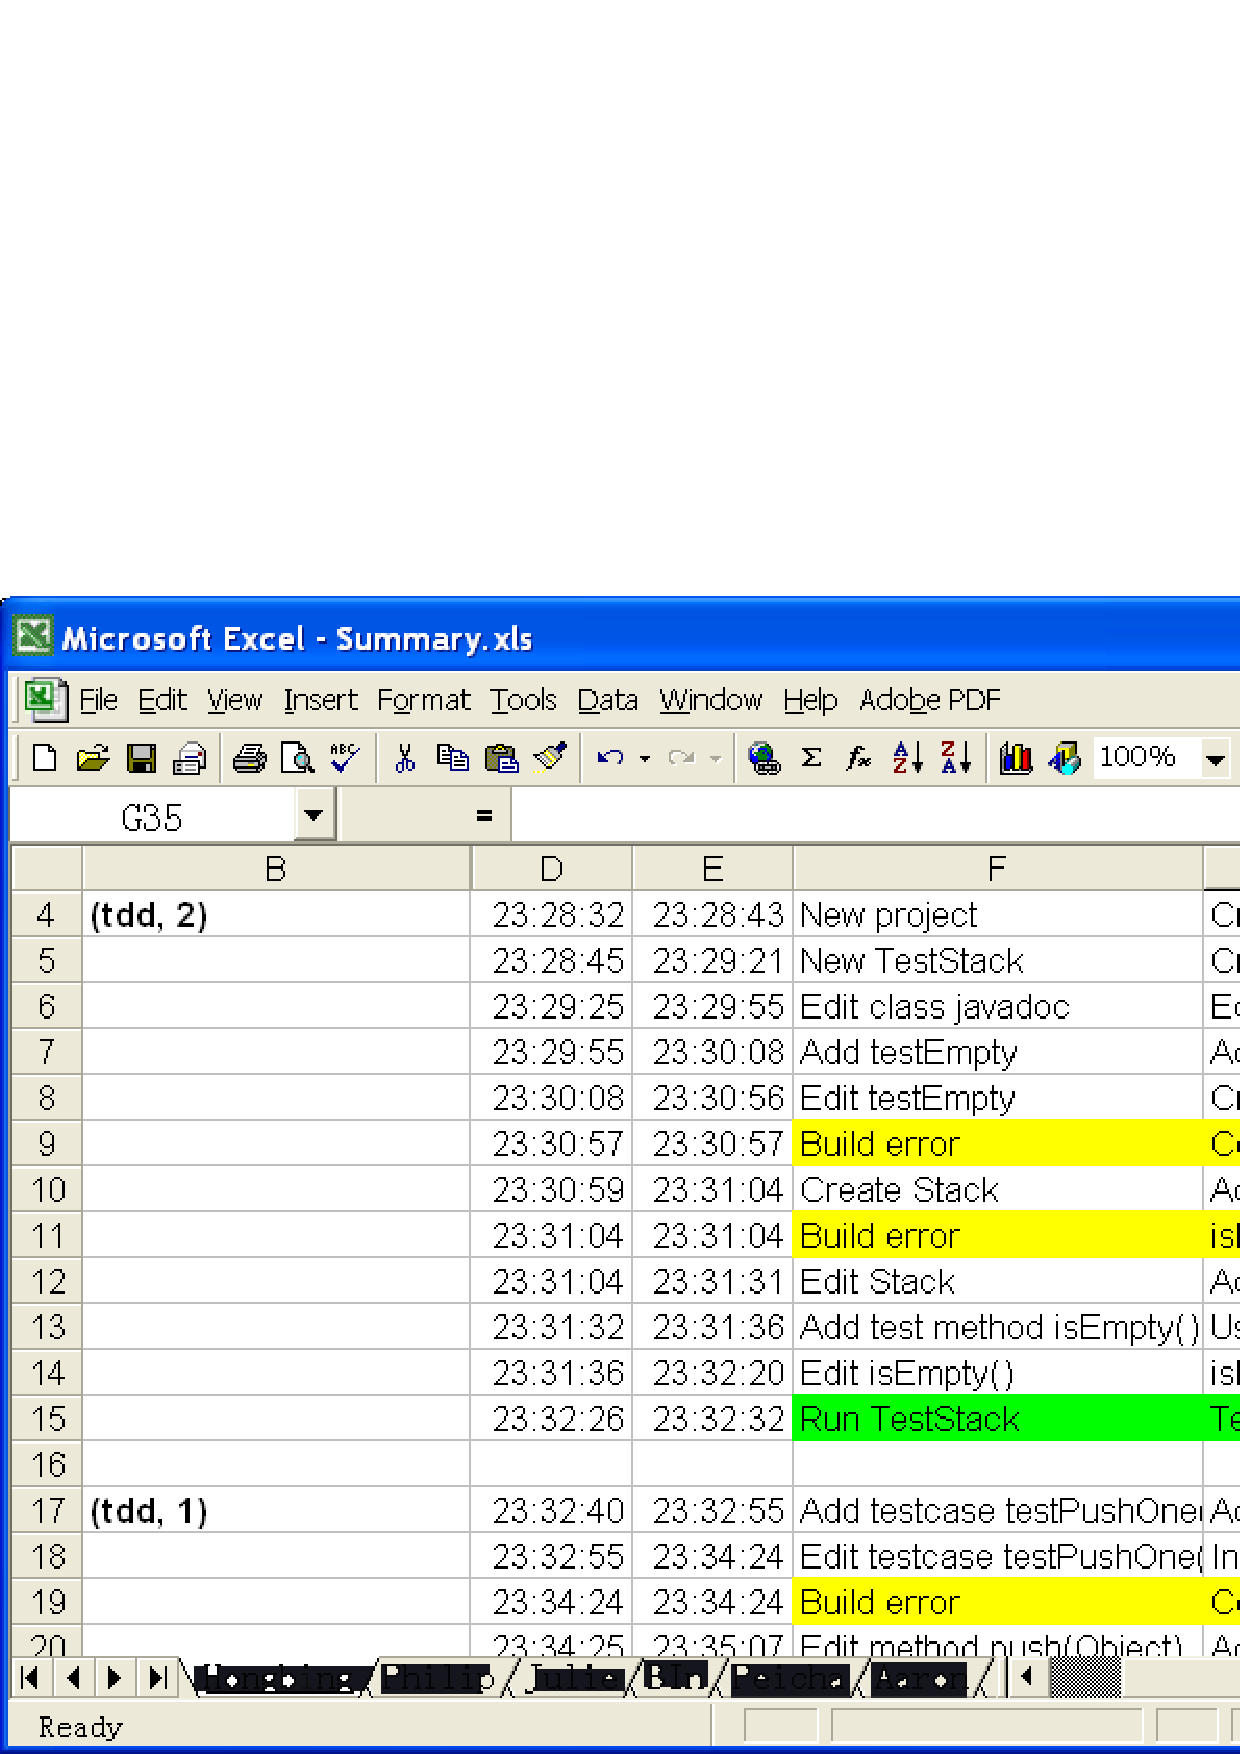
\includegraphics[width=1.0\textwidth]{VideoScriptExcel}
  \caption{Validation data in Excel}
  \label{fig:VideoExcelScript}
\end{figure}

We then checked for consistency: that the inferences made by Zorro matched
the behaviors we saw in the video, and whether there were TDD behaviors in
the video that Zorro did not capture.

{\bf Results.}  The participants spent between 28 and 66 minutes to
complete the task.  Zorro partitioned the overall development effort into
92 distinct episodes, out of which 86 were classified as either
Test-Driven, Refactoring, or Test-Last; the remainder were
``unclassified'', which normally corresponded to startup or shutdown
activities.  Note that the version of Zorro used in Spring 2006 used a
somewhat less sophisticated classification ruleset than the current
version. Table \ref{tab:EsrPilotStudy} provides a summary of these
validation results. For each subject (ID), the table shows the total number
of episodes inferred by Zorro, the number of correctly classified episodes
based upon ESR validation, and the resulting percentage correctly
classified, ordered from highest to lowest.

\begin{table}[ht]
\centering
  \caption{Case Study 1: TDD Development Behavior Validation}
  \begin{tabular}{|r|r|r|r|}
  \hline
    ID & Episodes & Correct & Percentage \\ \hline
    5  & 16 &  15 & 94\% \\ \hline
    3  & 14 &  13 & 93\% \\ \hline
    4  & 14 &  13 & 93\% \\ \hline
    6  & 11 &  10 & 91\% \\ \hline
    7  &  9 &  8  & 89\% \\ \hline
    1  & 15 &  13 & 87\% \\ \hline
    2  & 13 &  10 & 77\% \\ \hline \hline
Total  & 92 & 82  & 89\% \\ 
  \hline
  \end{tabular}
  \label{tab:EsrPilotStudy}  
\end{table}

Out of the 92 episodes under study, 82 were validated as correctly
classified, for an overall accuracy rate of 89\%.  The range in percentage
correctness ranged from 94\% to 77\%.  Analysis of the differences between
Zorro inferences and the ESR data analyses indicated that some editing work
and test case invocations were not captured correctly by Zorro.  These
fixes were made prior to the second case study.

{\bf Limitations.}  The most significant threats to validity of this study
were the sample size, the sample population, and the nature of the problem.
The study had only seven participants, some of whom were not experienced
with TDD.  Perhaps the most significant threat was the toy nature of the
programming problem, which raised the possibility that we would not be
observing ``real world'' software development behaviors with their
attendent complexities.

\subsection{Experiment 2: Classroom case study}

{\bf Goals.}  After improving the Zorro data collection and analysis
mechanisms based upon our first case study, we conducted a second case
study in the Fall of 2006.  The goal of this case study was to obtain
better quality data regarding the strengths and limitations of Zorro for
TDD inference by extending our experimental design to include direct
participant evaluation of Zorro inferences.

{\bf Procedure.}  We obtained agreement from 11 senior and graduate-level
students in two software engineering classes at the University of Hawaii.
These students had all recently completed a unit of test driven development
in their class, and had done a sample program using TDD principles.

The experimental session lasted approximately two hours. During the first
90 minutes, the students were given a brief introduction to the goals and
purpose of the study, then asked to work on the ``Bowling Score Keeper'', a
programming problem used in other empirical studies on TDD
\citep{George:03,Erdogmus:05}.  A set of user stories were provided to the
students to avoid the need for them to know the rules of scoring in
bowling, and also to provide them with a ``To Do'' list for programming.
The students were stopped at the end of 90 minutes regardless of whether or
not they had completed the entire programming problem.

Once the students finished the programming part of the experiment, they
were given a five minute break and then asked to validate Zorro's
inferences.  To do this, we implemented a special Zorro analysis that would
display a representation of each episode and allow the students to provide
feedback regarding their agreement with the analysis.  Figure
\ref{fig:EpisodeFeedback} shows an example of this wizard.

\begin{figure}[htbp]
  \centering
  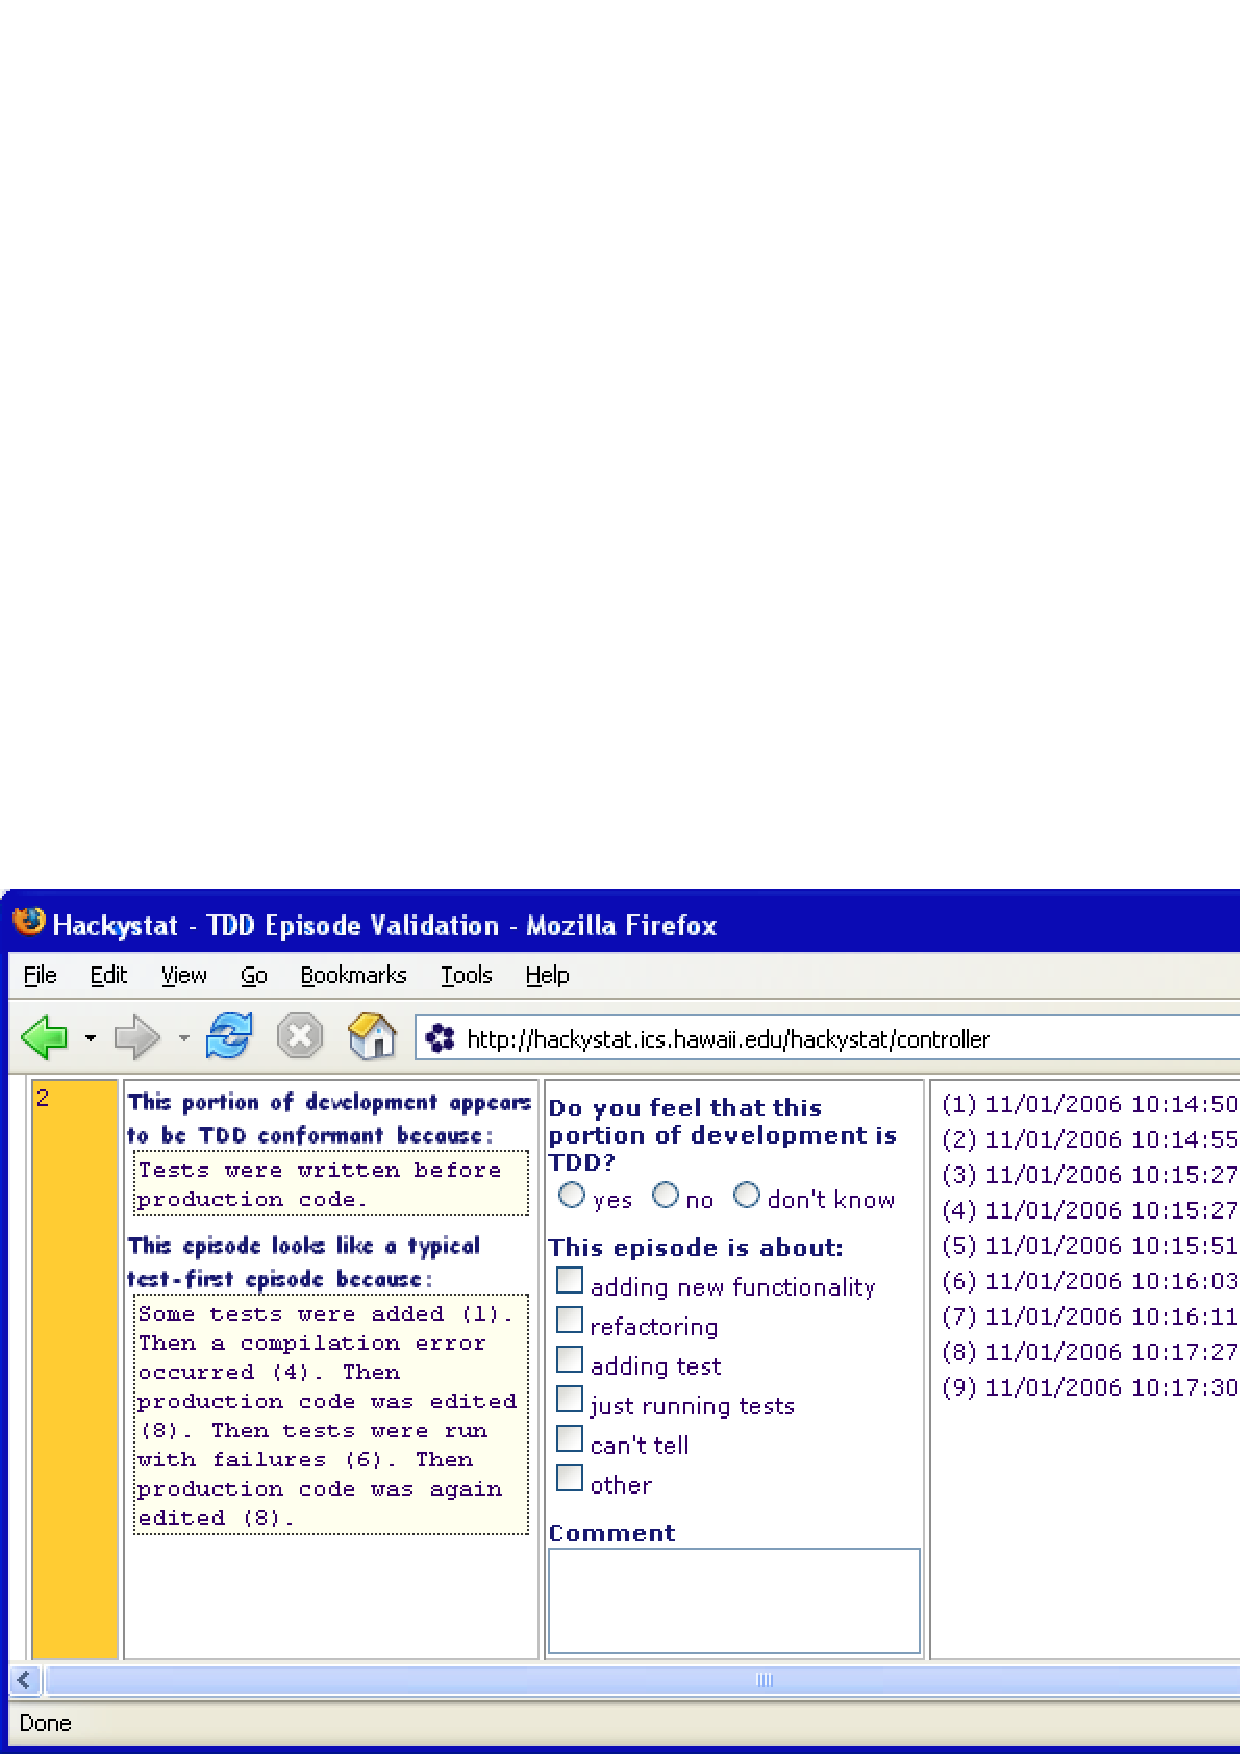
\includegraphics[width=1.0\textwidth]{EpisodeFeedback}
  \caption{TDD Episode Validation}\label{fig:EpisodeFeedback}
\end{figure}

To analyze the data, we repeated the same process of comparing Zorro analyses to the ESR video as in the first case study.  In addition, we also had the subject validation data, which provided a second independent source of information regarding the validity of Zorro inference.  

{\bf Results.}  The much richer data set collected in this data set makes possible a wide variety of analyses; for a full description, please see \cite{csdl2-07-04}.  In this section we present only a summary of the results. 

First, due to a bug in the data collection mechanism, we lost some data
from one participant. We decided to exclude this subject's data from further analysis, reducing our subject pool to 10. 


Table \ref{tab:EpisodeBehaviorAgreed} provides a summary of the validation results. For each subject (ID), the table lists the number of episodes inferred by Zorro, and the number of those episodes that were correctly classified based upon ESR video data and participant feedback, and the percentage that were correctly classified, ordered from highest to lowest.

\begin{table}[ht]
\centering
  \caption{Case Study 2: TDD Development Behavior Validation}
  \begin{tabular}{|r|r|r|r|}
  \hline
    ID & Episodes  & Correct & Percentage \\ \hline
    O       & 16   &  15   & 94\% \\ \hline
    R       & 14   &  13   & 93\% \\ \hline
    L       &  8   &   7   & 88\% \\ \hline  
    K       & 10   &   8   & 80\% \\ \hline
    A       & 19   &  15   & 79\% \\ \hline  
    T       & 13   &   9   & 69\% \\ \hline
    P       & 18   &  12   & 67\% \\ \hline
    Q       & 21   &  11   & 52\% \\ \hline
    N       &  9   &   4   & 44\% \\ \hline
    S       &  9   &   2   & 22\% \\ \hline
    Total   & 137  &  96   & 70\% \\ \hline
    \end{tabular}
  \label{tab:EpisodeBehaviorAgreed} 
\end{table}

These results are significantly worse than the first case study: the
overall percentage of correctness has dropped from 89\% to 70\%, and the
worst case performance dropped from 77\% to 22\%!

Analysis of the ESR video data and participant feedback revealed an
unexpected developer behavior which appears to account for much of the
difference in results between the two studies.  In Eclipse, it is possible
to invoke unit tests even when the production code does not
compile. Eclipse will issue a warning, but the developer can choose to
ignore it and run the tests anyway as long as the non-compiling code is not
actually invoked by the test cases.  Invoking tests on non-compiling
code is a violation of TDD principles, and had not occurred in our usage
of Zorro prior to this experiment. Zorro's rules were not configured to
deal with this situation, and as a result, 24 out of the 41 incorrectly
classified episodes contained an occurrence of this phenomena.

There are two ways to approximate the impact of this developer behavior on
Zorro's inference accuracy.  First, if we include only those developers who
never invoked unit tests when their code did not compile (i.e. the four top
subjects K, L, O, R), then the average percentage correctness of episode
inference is 90\%. Alternatively, if we exclude the 24 episodes in which
this phenomena was present from analysis, then the average percentage
correctness is 85\%.  These two approaches together provide some evidence that this
single behavior bears significant responsibility for the drop in overall accuracy
from the first study.

We can propose two ways to deal with this phenomena in future.  First, we
could adjust Zorro's current set of rules and/or sensors to take into
account the fact that some developers might wish to run unit tests in the
presence of non-compiling code. In this case, we would need to make a
decision about whether such a behavior would be TDD conformant or not.
Alternatively, and more simply, we could recommend that developers
intending to apply TDD principles configure Eclipse to disallow this
behavior.  We believe that the second approach is both easier and more
congruent with the current understanding of TDD practice.

In addition to this source of error, our analysis of the data discovered
several more minor problems. In two episodes, developers implemented trivial
changes to production code but did not run unit tests. The subjects claimed
that their behavior was TDD conformant, but without the invocation of test
cases, Zorro could not provide the appropriate episode boundary.  In four
episodes, developers defined a unit test method header, then wrote
production code, then wrote the unit test body.  Zorro's inference rules
were not able to handle a unit test whose initial definition was intermixed
with production code editing. Finally, in four episodes, Zorro initially
and incorrectly classified test code as production code since Zorro
requires assertions in the method body in order to recognize it as a test. 

{\bf Limitations.}  As with the first study, a primary threat to the
validity of this study is the small sample size.  In addition, the use of a
student population might influence the external validity of the findings,
as professional developers might behave differently than these students.
Another threat to external validity is the use of the Bowling Game
software problem, which is well suited to laboratory settings but not
necessarily representative of real-world software development. 

While participant-based validation of Zorro's inferences was quite helpful
in detecting certain problems, the views of participants, particularly
those with limited experience in TDD, must be taken with care.  It is
possible that at least some of the subjects felt that the software might
know better than they whether or not they were doing TDD.  

One way to address these limitations is to break out of the classroom
experimental paradigm, which we attempted to do in our third experiment
associated with this research.



\section{Contributions, limitations and future directions}
\label{sec:conclusions}

This research contributes in the following ways to the research and
practice of test-driven development in particular, and automated software
engineering in general.

First, to our knowledge, Zorro is the first, and so far only,
fully-automated system capable of recognizing test-driven development
practices.  Such a system can address the 
process compliance problem from which much current TDD research suffers. 

Second, by providing fully automated recognition, Zorro provides the first
precise, operational definition of TDD practice.  Our research revealed
that this operational definition was not straightforward to implement, as
certain kinds of episode types were intrinsicially ambiguous.  Resolving
these episode types required the implementation of disambiguation
heuristics. Our empirical evaluations demonstrated that these heuristics
seemed satisfactory in most situations, and that TDD episode recognition
accuracy of between 85-90\% is quite feasible.

Third, this research results in a new approach to measuring TDD compliance
based upon ``episodes'', or short-duration intervals of development.  Using
Zorro, one can speak of a development team as having used TDD ``55\% of the
time during the previous week''.  This much more fine-grained
characterization enables new kinds of research on TDD, such as whether
there is a threshold for TDD use.  For example, perhaps productivity and
quality do climb with TDD use up to a threshold of, say, 80\%, beyond which
there is no discernable improvement.  As another example, perhaps there is
a steep drop-off in quality and/or productivity if TDD usage drops below,
say, 30\%.

The Zorro system was implemented within the Software Development
Stream Analysis (SDSA) framework.  SDSA provides a generic means for
recognition of developer ``micro-processes'' such as TDD.  In future work,
we hope to write new applications on top of SDSA in addition to Zorro, such
as an application for recognizing Continuous Integration best practices.

The external validity of our first two case studies is
threatened by the use of students in a classroom setting.  To address this
threat, we hoped to gain insight into the usefulness of Zorro in an 
industrial setting in collaboration with an external research partner. 
We ported the Eclipse Zorro sensor to Visual Studio and TestDriven.NET for 
this purpose.  20 professional developers were recruited 
by our external partner from a European company, but it was not possible to 
have on-site researcher
presence during the study. Unfortunately, we could not collect 
sufficient and reliable data due to factors outside our control to triangualte 
our results from student experiments. Future efforts will focus on 
redesigning and conducting studies with professional developers to further 
validate and improve TDD inference capabilities. We realize that 
 researcher access to participants and their programming environments is 
critical for ensuring consistent and reliable data collection.  

\begin{acknowledgements}
We gratefully acknowledge the members of the Collaborative Software 
Development Laboratory who supported this research, 
as well as the student and industrial participants in the evaluation.  
The Software Engineering Group of the National Reseach Council of Canada participated 
in this research
under a cooperative agreement. 
Dr. Burak Turhan of NRC provided valuable comments and information regarding
tool support for TDD adoption.

\end{acknowledgements}

\bibliographystyle{spbasic}      % basic style, author-year citations
% The \cite command functions as follows:
 %   \citet{key} ==>>                Jones et al. (1990)
 %   \citet*{key} ==>>               Jones, Baker, and Smith (1990)
 %   \citep{key} ==>>                (Jones et al., 1990)
 %   \citep*{key} ==>>               (Jones, Baker, and Smith, 1990)
 %   \citep[chap. 2]{key} ==>>       (Jones et al., 1990, chap. 2)
 %   \citep[e.g.][]{key} ==>>        (e.g. Jones et al., 1990)
 %   \citep[e.g.][p. 32]{key} ==>>   (e.g. Jones et al., p. 32)
 %   \citeauthor{key} ==>>           Jones et al.
 %   \citeauthor*{key} ==>>          Jones, Baker, and Smith
 %   \citeyear{key} ==>>             1990
\bibliography{tdd,zorro,csdl-trs,hackystat,psp}
\end{document}

